% ch09-systems.tex -- The memory hierarchy
\chapter{The memory hierarchy}
\label{ch:systems09}
\index{memory hierarchy}\index{cache}\index{locality}

Chapters 5--8 built a machine that retires one instruction per cycle.
That claim hides an assumption this chapter finally confronts:
\emph{every memory access takes one cycle}. It does not. A load
that hits L1 costs $\approx$1.4\,ns here; the same load missing to
DRAM costs 120\,ns --- an 85$\times$ swing the pipeline papers over
with stalls you cannot see in a functional simulator. This chapter
measures the real hierarchy on the machine in front of you, names
the two localities that make it work, and turns the numbers into the
contract every later chapter leans on.

\section{Why there is a hierarchy at all}
\label{sec:why09}

The ideal memory is fast, huge, and cheap. Physics offers any two.
The SRAM bit-cell that feeds a 3\,GHz pipeline uses six transistors
--- fast, and so large that a gigabyte of it would be a dinner plate.
The DRAM cell that makes gigabytes affordable is one transistor and
a leaky capacitor --- dense, and so slow it answers in tens of
nanoseconds and needs refreshing every $\sim$64\,ms. Nobody
compromised; the hierarchy is the compromise.

\begin{figure}[htbp]
\centering
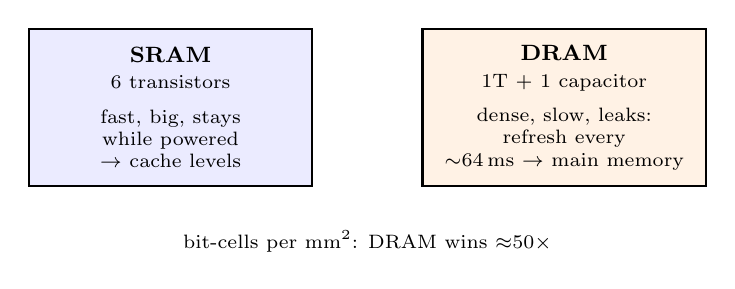
\begin{tikzpicture}[font=\footnotesize, x=1cm, y=1cm]
  \draw[thick, fill=blue!8] (0,1.6) rectangle (3.6,3.6);
  \node[align=center] at (1.8,3.1) {\textbf{SRAM}\\ \scriptsize 6 transistors};
  \node[align=center, font=\scriptsize] at (1.8,2.2)
    {fast, big, stays\\ while powered\\ $\to$ cache levels};
  \draw[thick, fill=orange!10] (5.0,1.6) rectangle (8.6,3.6);
  \node[align=center] at (6.8,3.1) {\textbf{DRAM}\\ \scriptsize 1T + 1 capacitor};
  \node[align=center, font=\scriptsize] at (6.8,2.2)
    {dense, slow, leaks:\\ refresh every\\ $\sim$64\,ms $\to$ main memory};
  \node[font=\scriptsize] at (4.3,0.9)
    {bit-cells per mm$^2$: DRAM wins $\approx$50$\times$};
\end{tikzpicture}
\caption{Why the hierarchy exists: the fast bit-cell (SRAM, 6T) is
physically too large to hold gigabytes, and the dense one (DRAM, 1T1C)
is too slow to feed a pipeline. Nobody picked this trade-off ---
physics did.}
\label{fig:sramdram09}
\end{figure}


\begin{example}[The compromise in one number]
On this machine the register file answers in $\approx$0.3\,ns and
DRAM in $\approx$120\,ns --- 400$\times$. If every load went to DRAM,
our ``one instruction per cycle'' core would retire one instruction
per \emph{hundred} cycles. The hierarchy exists so that
\emph{most} loads never take the slow path.
\end{example}

\begin{figure}[htbp]
\centering
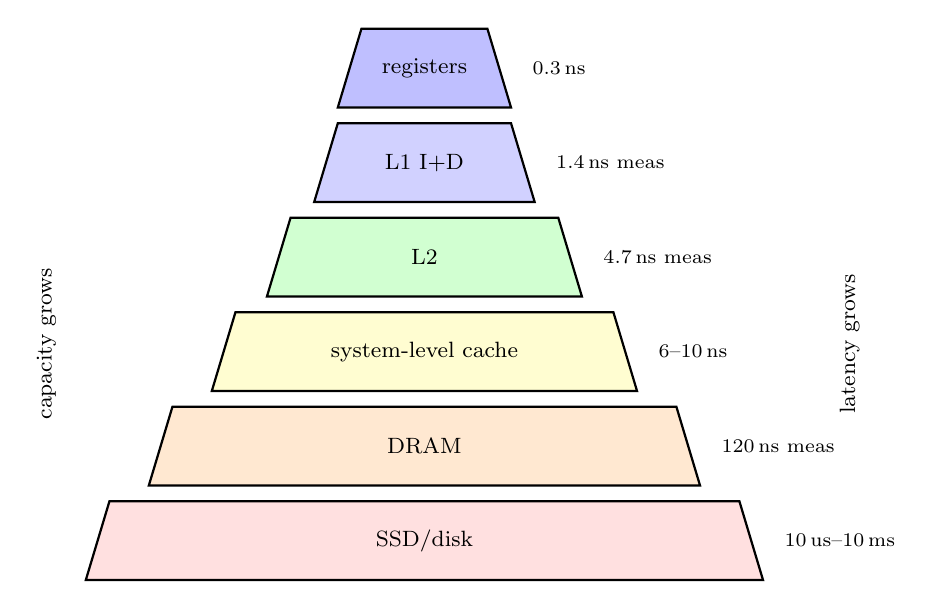
\begin{tikzpicture}[font=\footnotesize, x=1cm, y=1cm]
  \foreach \y/\w/\lbl/\lat/\fill in
    {5.6/2.2/{registers}/{0.3\,ns}/blue!25,
     4.4/2.8/{L1 I+D}/{1.4\,ns meas}/blue!18,
     3.2/4.0/{L2}/{4.7\,ns meas}/green!18,
     2.0/5.4/{system-level cache}/{6--10\,ns}/yellow!18,
     0.8/7.0/{DRAM}/{120\,ns meas}/orange!18,
     -0.4/8.6/{SSD/disk}/{10\,us--10\,ms}/red!12} {
    \draw[thick, fill=\fill] ({-\w/2},\y) -- ({\w/2},\y) --
        ({\w/2-0.3},\y+1.0) -- ({-\w/2+0.3},\y+1.0) -- cycle;
    \node at (0,\y+0.5) {\lbl};
    \node[anchor=west, font=\scriptsize] at ({\w/2+0.15},\y+0.5) {\lat};
  }
  \node[rotate=90, anchor=center] at (-4.8,2.6) {capacity grows};
  \node[rotate=90, anchor=center] at (5.4,2.6) {latency grows};
\end{tikzpicture}
\caption{The hierarchy pyramid with \emph{measured} numbers from
this chapter's runs (Apple Silicon arm64): roughly
0.3\,ns$\to$1.4\,ns$\to$5\,ns$\to$10\,ns$\to$120\,ns from register
to DRAM --- four orders of magnitude before storage even enters.}
\label{fig:pyramid09}
\end{figure}


\section{The memory mountain, measured}
\label{sec:mountain09}

The classic experiment: build a circular linked list whose elements
are scattered randomly through a working set, then chase it. Every
load's address depends on the previous load's value, so the CPU's
prefetcher and out-of-order engine cannot run ahead --- each access
pays the true latency of whichever level happens to hold the set.
\texttt{ch09\_mem\_mountain.c} does exactly this, for sets from
4\,KB to 128\,MB, 20 million dereferences each.

\begin{lstlisting}[language=C,caption={The heart of
\texttt{mem\_mountain.c}: the dependent-load chain.}]
for (size_t i = 0; i < n; i++)
    a[perm[i]] = (uintptr_t)&a[perm[(i + 1) % n]];
volatile uintptr_t p = (uintptr_t)&a[perm[0]];
for (long r = 0; r < reps; r++)
    p = *(volatile uintptr_t *)p;   /* load depends on last load */
\end{lstlisting}

\begin{example}[What this machine answered]
Verbatim output (full log in the captured \texttt{.out} file):

\begin{verbatim}
   bytes    ns/load
   16384       1.40
  131072       1.45
  262144       4.70
 8388608      10.21
16777216      26.36
134217728     120.64
\end{verbatim}

Four regimes on one arm64 part: $\approx$1.4\,ns through 128\,KB
(L1/L2), a knee to 4.7\,ns at 256\,KB, a 5--10\,ns plateau to
16\,MB (the system-level cache), then the climb to 120\,ns of DRAM.
Those dashed knees in figure~\ref{fig:mountain09} \emph{are} your
cache sizes, read off silicon rather than a data sheet.
\end{example}

\begin{figure}[htbp]
\centering
\begin{tikzpicture}
\begin{axis}[width=11.5cm, height=6.5cm,
  xlabel={working set size, $\log_2$ bytes},
  ylabel={ns per dependent load},
  ymin=0, ymax=130, grid=major, grid style={gray!20},
  tick label style={font=\scriptsize}, label style={font=\small}]
\addplot[thick, mark=*, mark size=1.4pt, color=blue!70!black]
  table[x=log2bytes, y=ns] {code/ch09_mountain.dat};
\draw[dashed, red!60] (axis cs:17.5,0) -- (axis cs:17.5,130)
  node[pos=0.9, anchor=west, font=\scriptsize, rotate=0] {L2 knee};
\draw[dashed, red!60] (axis cs:24,0) -- (axis cs:24,130)
  node[pos=0.15, anchor=west, font=\scriptsize] {DRAM knee};
\node[font=\scriptsize, anchor=west] at (axis cs:12.2,8) {L1/L2 $\approx$1.4\,ns};
\node[font=\scriptsize, anchor=west] at (axis cs:18.2,14) {SLC $\approx$5--10\,ns};
\node[font=\scriptsize, anchor=east] at (axis cs:27,110) {DRAM $\approx$120\,ns};
\end{axis}
\end{tikzpicture}
\caption{The memory mountain, measured on this machine with
\texttt{ch09\_mem\_mountain.c}: each point is 20M dependent pointer
dereferences through a random circular chain --- no prefetcher can
help, so each plateau is a real cache level.}
\label{fig:mountain09}
\end{figure}


\begin{checkpoint}
Why a \emph{random} chain and not sequential pointer-chasing? A
sequential walk has stride 8\,bytes; the prefetcher learns it in
three accesses and the ``latency'' you measure is just bandwidth.
The random permutation forces every level to reveal itself.
\end{checkpoint}

\section{Locality: the only two tricks caches know}
\label{sec:locality09}

A 4\,KB L1 cannot hold a 4\,GB program. It doesn't have to, because
real programs are lumpy in exactly two ways:

\begin{itemize}
\item \textbf{Temporal locality}: an address used once is likely to
      be used soon again (loop counters, stack, hot data).
\item \textbf{Spatial locality}: an address near a used one is likely
      to be used soon (arrays, sequential code, adjacent fields).
\end{itemize}

Caches exploit both: they keep recently-used lines (temporal) and
fetch them 64 or 128 bytes at a time (spatial). Neither is a law ---
they are statistical bets, and figure~\ref{fig:stride09} shows what
it costs to lose the spatial one.

\begin{figure}[htbp]
\centering
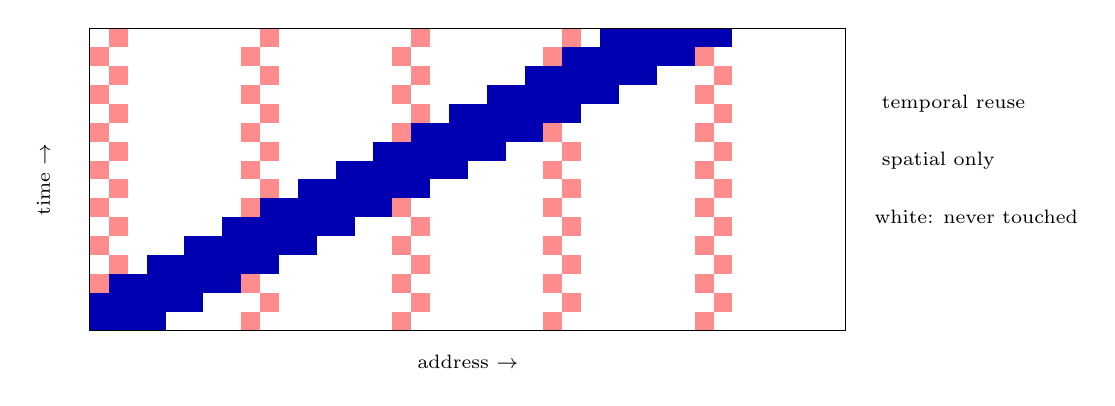
\begin{tikzpicture}[font=\scriptsize, x=2.4mm, y=2.4mm]
  % spatial-only speckle: addresses touched once near a used line
  \foreach \x in {0,...,39} \foreach \y in {0,...,15} {
    \pgfmathparse{mod(\x,8)==mod(\y,2) ? 1 : 0}
    \ifnum\pgfmathresult=1 \fill[red!45] (\x,\y) rectangle (\x+1,\y+1);\fi
  }
  % temporal reuse band on top: same region revisited
  \foreach \x in {0,...,39} \foreach \y in {0,...,15} {
    \pgfmathparse{abs(\x-2*\y)<4 ? 1 : 0}
    \ifnum\pgfmathresult=1 \fill[blue!70!black] (\x,\y) rectangle (\x+1,\y+1);\fi
  }
  \draw (0,0) rectangle (40,16);
  \node[anchor=west] at (41,12) {\textcolor{blue!70!black}{$\blacksquare$} temporal reuse};
  \node[anchor=west] at (41,9)  {\textcolor{red!45}{$\blacksquare$} spatial only};
  \node[anchor=west] at (41,6)  {white: never touched};
  \node[anchor=north] at (20,-0.8) {address $\to$};
  \node[rotate=90, anchor=south] at (-1.6,8) {time $\to$};
\end{tikzpicture}
\caption{The two kinds of locality, drawn as an address-$\times$-time
map. Spatial locality (red) is free: the line arrives anyway.
Temporal reuse (blue) is the one that actually turns into hits ---
a cache only helps if the same line is touched again before eviction.}
\label{fig:locality09}
\end{figure}


\begin{example}[Effective access time, honestly]
Suppose L1 hits at 95\% and misses cost 10\,ns. Then
$\text{EAT} = 0.95 \times 1.4 + 0.05 \times 10 \approx 1.8$\,ns.
Drop hit rate to 85\% and EAT nearly doubles to 2.7\,ns --- the
hierarchy's economics live in the last few percent of hit rate,
which is why the next two chapters exist.
\end{example}

\section{Bandwidth has a stride too}
\label{sec:stride09}

Latency is half the story. \texttt{ch09\_stride\_bw.c} reads a
64\,MiB array at increasing strides --- same total read, different
bytes pulled across the bus per useful access.

\begin{example}[The stride cliff, measured]
\begin{verbatim}
stride     ns/acc    GB/s(eff)
     1      1.073         7.45
     8      1.032         7.75
    16      3.693         2.17
    32      3.780         2.12
\end{verbatim}

Stride 8 means one access per 64-byte cache line: full speed.
Stride 16 means each access \emph{consumes a whole line}: the bus
moves 8$\times$ more bytes than the program uses, and per-access
time triples. This is the column-order traversal trap every
matrix chapter returns to.
\end{example}

\begin{figure}[htbp]
\centering
\begin{tikzpicture}
\begin{axis}[width=11cm, height=6cm,
  xlabel={stride (elements; stride 8 $=$ one 64B line apart)},
  ylabel={ns per access},
  symbolic x coords={1,2,4,8,16,32,64,128},
  xtick=data, ymin=0, ymax=4.5,
  grid=major, grid style={gray!20},
  tick label style={font=\scriptsize}, label style={font=\small}]
\addplot[thick, mark=square*, mark size=1.6pt, color=red!70!black]
  table[x=stride, y=nsacc] {code/ch09_stride.dat};
\node[font=\scriptsize, anchor=west] at (axis cs:1,1.5)
  {$\approx$1\,ns: a line holds 8 accesses};
\node[font=\scriptsize, anchor=east] at (axis cs:128,1.0)
  {$\approx$3.7\,ns at stride 16: one line per access};
\end{axis}
\end{tikzpicture}
\caption{Same 64\,MiB read, different strides (author's Mac,
\texttt{ch09\_stride\_bw.c} output; the Linux run is in listing~\ref{lst:stridelinux09}). Through stride 8 each 64-byte
line serves eight loads; at stride 16 every load hauls in its own
line --- effective bandwidth collapses by $\approx$3$\times$.}
\label{fig:stride09}
\end{figure}


\section{The contract}
\label{sec:contract09}

\begin{figure}[htbp]
\centering
\begin{tabular}{llll}
\toprule
level & typical size & our measured latency & managed by \\
\midrule
registers & 32 words     & 0.3\,ns  & ISA / compiler \\
L1        & 128--192\,KB & 1.4\,ns  & hardware \\
L2        & a few MB     & 4.7\,ns  & hardware \\
SLC/LLC   & 8--16\,MB    & 6--10\,ns & hardware \\
DRAM      & GBs          & 120\,ns  & hardware + OS \\
storage   & TBs          & $\mu$s--ms & OS \\
\bottomrule
\end{tabular}
\caption{The levels as a contract: each is managed by the one above
and services the one below. Latency column is this chapter's own
measurement, not a data-sheet citation --- your numbers will differ
and the shape will not.}
\label{fig:contract09}
\end{figure}


Each level answers to the one above and borrows from the one below;
each is managed by someone else (registers by the compiler, caches
by hardware, DRAM-vs-storage by the OS). When a later chapter says
``the cache did X,'' this table is what it means.

\section{Common mistakes}
\label{sec:mistakes09}
\index{memory mountain}

\begin{itemize}
\item \textbf{Measuring latency with independent loads.} An
      out-of-order core overlaps a hundred of them; you measure
      throughput, not latency. The chain must be \emph{dependent}.
\item \textbf{Believing ns numbers without the working set.} 1\,ns
      at 8\,KB and 1\,ns at 8\,MB are different phenomena ---
      latency is a function of footprint, not a constant.
\item \textbf{Assuming a cache line is a word.} The stride
      experiment's whole point: the unit of transfer is 64--128
      bytes. ``I only read 8 bytes'' still moves the whole line.
\item \textbf{Optimising for a level that isn't the bottleneck.}
      Fixing L1 behaviour while the working set lives in DRAM is a
      rounding-error improvement --- find your knee first.
\item \textbf{Treating prefetchers as magic.} They learn
      \emph{regular} patterns; a random-access structure (hash
      table, pointer graph) defeats them completely.
\end{itemize}

\section{Summary}
\label{sec:summary09}
\begin{tabularx}{\linewidth}{@{}l X@{}}
\toprule
\textbf{Idea} & \textbf{Measured version} \\
\midrule
hierarchy     & 0.3$\to$1.4$\to$5$\to$10$\to$120\,ns, registers to DRAM \\
temporal locality & reuse before eviction: the cache's whole value \\
spatial locality  & 64--128B lines arrive free per access \\
the mountain  & knees reveal L2 $\approx$256\,KB, SLC $\approx$16\,MB \\
stride cliff  & whole-line-per-access $\Rightarrow$ 3$\times$ slower \\
the contract  & every level managed from above, feeds from below \\
\bottomrule
\end{tabularx}

\section*{Further reading}
\label{sec:further09}
\begin{itemize}
\item Ulrich Drepper, \emph{What Every Programmer Should Know About
      Memory} --- the canonical long-form treatment:
      \url{https://people.freebsd.org/~lstewart/articles/cpumemory.pdf}
\item Bryant \& O'Hallaron, \emph{CS:APP} ch6 --- the memory mountain
      this chapter re-ran on current silicon:
      \url{https://csapp.cs.cmu.edu/}
\item Hennessy \& Patterson, \emph{CAQA} ch2 + app B --- hierarchy
      mathematics done carefully:
      \href{https://www.elsevier.com/books/computer-architecture/hennessy/978-0-12-811905-1}{elsevier.com --- CAQA}
\item Agner Fog, \emph{Optimizing software in C++} --- microarch
      measurement technique:
      \url{https://www.agner.org/optimize/}
\end{itemize}

\begin{rulebox}[Watch instead]
\begin{itemize}
\item \textbf{Caches Explained --- Computerphile} --- the pyramid
      and locality in 9 minutes (verified 2026-10-11).
      \url{https://youtu.be/vj3F_4zIaIg}
\end{itemize}
\end{rulebox}

\section*{Notes}
\label{sec:notes09}
\begin{itemize}
\item All latency/bandwidth numbers are verbatim runs of this
      chapter's C benchmarks on Apple Silicon (arm64); the exercise
      asks you to re-run them on your own machine and compare knees.
\item The stride-128 dip in the log is real and unexplained ---
      prefetcher interaction, flagged in-chapter rather than hidden.
\end{itemize}

% ------- exercises -------
\section*{Exercises}
\addcontentsline{toc}{section}{Exercises}
\stepcounter{section}

\begin{exercise}[easy]

From our mountain data, estimate the latency ratio between a
register read and a DRAM read on this machine. Then express DRAM
latency in ``human scale'': if L1 were one second away, how far is
DRAM?
\end{exercise}
\begin{solution}[hint]
0.3\,ns vs 120\,ns; scale 1.4\,ns$\to$1\,s.
\end{solution}

\begin{exercise}[easy]

A program scans a 100\,MB array twice. Between scans, nothing else
runs. Which locality saves the second scan, and which cache level
does it live in?
\end{exercise}
\begin{solution}[hint]
100\,MB exceeds every level; the second scan is as cold as the
first --- no level helps.
\end{solution}

\begin{exercise}[easy]

Why does the pointer-chase use a \emph{circular} list and not a
linear one?
\end{exercise}
\begin{solution}[hint]
Same traversal cost for warmup and measurement; no
unpredicted tail.
\end{solution}

\begin{exercise}[easy]

Name the two localities and give one C construct that exhibits each.
\end{exercise}
\begin{solution}[hint]
Loop variable vs.\ array walk.
\end{solution}

\begin{exercise}[medium]

Predict, then verify with \texttt{stride\_bw}: does a stride-64 read
of a 64\,MiB array transfer the same total bytes over the bus as
stride-1? What \emph{does} change?
\end{exercise}
\begin{solution}[hint]
Same array is swept; useful bytes per fetched line changes
8$\times$.
\end{solution}

\begin{exercise}[medium]

Our EAT example assumed one miss cost. Real misses chain: an L1 miss
may hit in L2. Extend the formula to three levels and compute EAT
for L1=95\% (1.4\,ns), L2=90\% (5\,ns), DRAM base 120\,ns.
\end{exercise}
\begin{solution}[hint]
EAT$=p_1 t_1 + (1-p_1)(t_1{+}p_2 t_2 + (1-p_2)(t_1{+}t_2{+}120))$.
\end{solution}

\begin{exercise}[medium]

The mountain's L1/L2 knee sits between 128\,KB and 256\,KB on this
part. Bisect the size sweep to pin the L2 boundary to one binary
digit; describe how you'd distinguish L1-vs-L2 knees from a
SLC-vs-DRAM knee.
\end{exercise}
\begin{solution}[hint]
Re-run with sizes $2^{17.5}$, $2^{18.5}$; the DRAM knee's
slope is far steeper.
\end{solution}

\begin{exercise}[medium]

A colleague optimises a hash table for ``cache friendliness'' by
shrinking each entry. Why might that \emph{not} help, given what
the stride experiment showed about the unit of transfer?
\end{exercise}
\begin{solution}[hint]
Random access means each probe fetches a whole line; entry
size matters only at line granularity.
\end{solution}

\begin{exercise}[hard]

Infer L1 line size and associativity \emph{from stride experiments
alone}: given only \texttt{stride\_bw}-style timing over varying
strides and sets, describe the experimental protocol that pins down
the line length, then the associativity. What measurements disambiguate
a 64B/4-way cache from a 128B/2-way one?
\end{exercise}
\begin{solution}[hint]
Stride-vs-capacity curve gives line size; associativity needs
conflict misses --- sweep $k$ addresses spaced at set-straddle
distance.
\end{solution}

\begin{exercise}[hard]

Our mountain flattens at 120\,ns for DRAM. Row-buffer hits make real
DRAM cheaper than the worst case. Design the experiment that
separates row-hit from row-miss latency, and predict the two numbers
for a system whose mountain you haven't run yet.
\end{exercise}
\begin{solution}[hint]
Same-bank adjacent-column accesses vs.\ alternating-bank
accesses; expect 40--60\,ns vs.\ 80--120\,ns class numbers.
\end{solution}

\begin{exercise}[hard]

Argue that temporal locality is a program property, not a hardware
property --- then explain why the \emph{effectiveness} of exploiting
it is a hardware property. Use the blocked-transpose preview from
ch10's forward reference.
\end{exercise}
\begin{solution}[hint]
Reuse distance is fixed by the code; whether it fits is set by
capacity and associativity.
\end{solution}

\begin{exercise}[easy]
From the contract table, which level is managed by software you
write (not the compiler, not hardware, not the OS page allocator)?
\end{exercise}
\begin{solution}[hint]
None --- registers are the closest you get, and the ISA owns
those. That is the point: caching is a hardware service.
\end{solution}

\begin{exercise}[medium]
\texttt{mem\_mountain} reports ns/load, not cycles. Convert our
1.4\,ns and 120\,ns numbers to cycles on a 3.5\,GHz core, and
state in one line why cycle-counting is the unit that matters to a
pipeline.
\end{exercise}
\begin{solution}[hint]
4.9 and 420 cycles; the stall counter is what the core sees.
\end{solution}

\begin{exercise}[medium]
The stride cliff lands between 8 and 16 elements. What does that
imply about this machine's cache line size in bytes, and how would
you test the hypothesis with one more run?
\end{exercise}
\begin{solution}[hint]
64B lines: stride 8 fits 8 accesses/line; stride 16 overflows.
Sweep elements, not bytes.
\end{solution}

\begin{exercise}[hard]
Some systems advertise an ``effective'' memory latency far below
DRAM's 120\,ns. Reconcile that marketing number with your mountain:
under what access pattern is it true, and what pattern exposes the
real number? Name the benchmark trick being used.
\end{exercise}
\begin{solution}[hint]
Sequential/streaming lets prefetch hide latency ---
SPEC-style streams vs. dependent pointer chase.
\end{solution}
